\subsection{Обзор методов и алгоритмов решения поставленной задачи}

В курсовом проекте используется алгоритм шифрования и дешифрования, названный в честь ученого Дэвида Хаффмана, разработавшего его в ходе выполнения курсовой работы в Массачусетском технологическом институте в 1952 году.
Данный способ архивации относится к группе "жадных" алгоритмов, где принимаются локально оптимальные решения на каждом шаге, допуская конечное решение также оптимальным.
Он представляет собой процесс кодирования файла по словарю префиксных значений заданного выражения.



Идея, лежащая в основе кода Хаффмана\cite{wiki_huf}, достаточно проста. 
Вместо того чтобы кодировать все символы одинаковым числом бит (например, в ASCII кодировке на каждый символ отводится ровно по 8 бит), символам с большей частотой ставятся в соответствие более короткие коды.
Соответвенно редким символам будет соответствовать более длинный код.
В данном случая под кодом подразумеваются биты, используемые для представления конкретного символа или другой единицы объема информации.



Для однозначного шифрования символов (значение должно быть единственным) коды Хаффмана должны обладать свойством префиксности\cite{algo} -- каждое кодовое слово не должно быть префиксом другого.
Таким образом можно использовать для кодирования меньшее число бит, чем максимально возможное, а значит и эффективность сжатия возрастает.
Главное учитывать, что при такой архивации усложняется декодирование сжатой информации.



Стоит отметить, что такой алгоритм Хаффмана в первоначальном виде будет однозначно работать только с файлами, представляемыми в текстовом виде: .txt, .tex, .html, .cpp и другие форматы файлов преобразуемые в текст.
Если же попробовать закодировать нашим алгоритмом, например, изображение, результат может быть неопределенным, так как будет видоизменяться структура самого файла.



Алгоритм Хаффмана двухпроходный. На первом проходе строится частотный словарь и генерируются коды. 
На втором проходе происходит непосредственное кодирование всех символов.



При построении частотного словаря создается контейнер\cite{lafore} для записи значений (можно использовать последовательные или ассоциативные -- в данном случае реализация зависит только от предпочтений разработчика) и производится проход по файлу.
Во время чтения файла количество вхождений каждого символа исходного алфавита записывается в соответствующую ячейку контейнера для построения бинарного дерева поиска (H-дерево)\cite{algo}.

\begin{figure}[h]
    \centering
    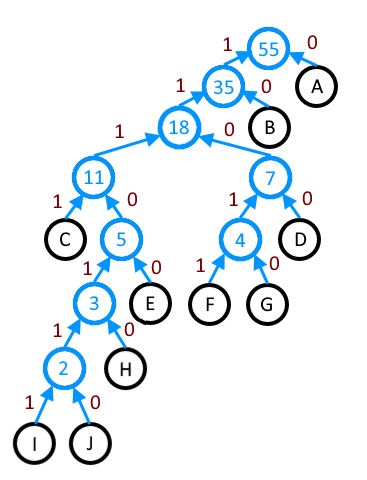
\includegraphics[height=8.5cm]{\commonSecPathPrefix/sec_2/content/example_tree.png}
    \caption{Пример построенного дерева Хаффмана}
    \label{fig:exmple_htree}
\end{figure}



Оптимальный код файла всегда будет представлен полным бинарным деревом (см. рис. \ref{fig:exmple_htree}), каждый узел (кроме листьев) которого имеет по два дочерних узла.
При отсутствии префиксности и использовании кодов одинаковой длины дерево становится неполным\cite{algo}, а значит и кодирование файла становится менее эффективным.



Дерево кодирования символов формируется из созданного ранее частотного словаря по следующему алгоритму:
\begin{enumerate}
    \item[1] Составляется список кодируемых символов (при этом каждый символ является одноэлементным бинарным деревом, вес которого равен весу символа и количеству вхождений этого символа в кодируемое сообщение).    
    \item[2] Выбираются два узла из списка с наименьшими весами.
    \item[3] Формируется новый узел и присоединяется к нему, в качестве дочерних, два узла выбранных из списка. При этом вес сформированного узла равен сумме весов дочерних узлов.
    \item[4] Сформированный узел добавляется к списку.
    \item[5] Если в списке больше одного узла, то повторить пункты 2-5.
\end{enumerate}



Таким образом при движении по дереву от корня к листьям у нас образуется кодировка символа, находящегося в листе дерева.
По этому дереву строится контейнер, содержащий кодировки всех символов алфавита.
Используя данные из контейнера кодируется вся исходная последовательность.



Чтобы правильно декодировать уже сжатый файл, в его начало записывается таблица частот алфавита и уже по ней расшифровывается закодированная последовательность, записанная после таблицы.



Именно из-за записи частотной таблицы архивация становится менее эффективной. 
Если же не учитывать длину этой таблицы, то длина сжатого файла всегда будет меньше либо равной первоначальной.
Обычно в таких случаях, только при записи закодированных данных, сжатие позволяет сэкономить от 20\% до 90\% объема информации.



\begin{figure}[h]
    \centering
    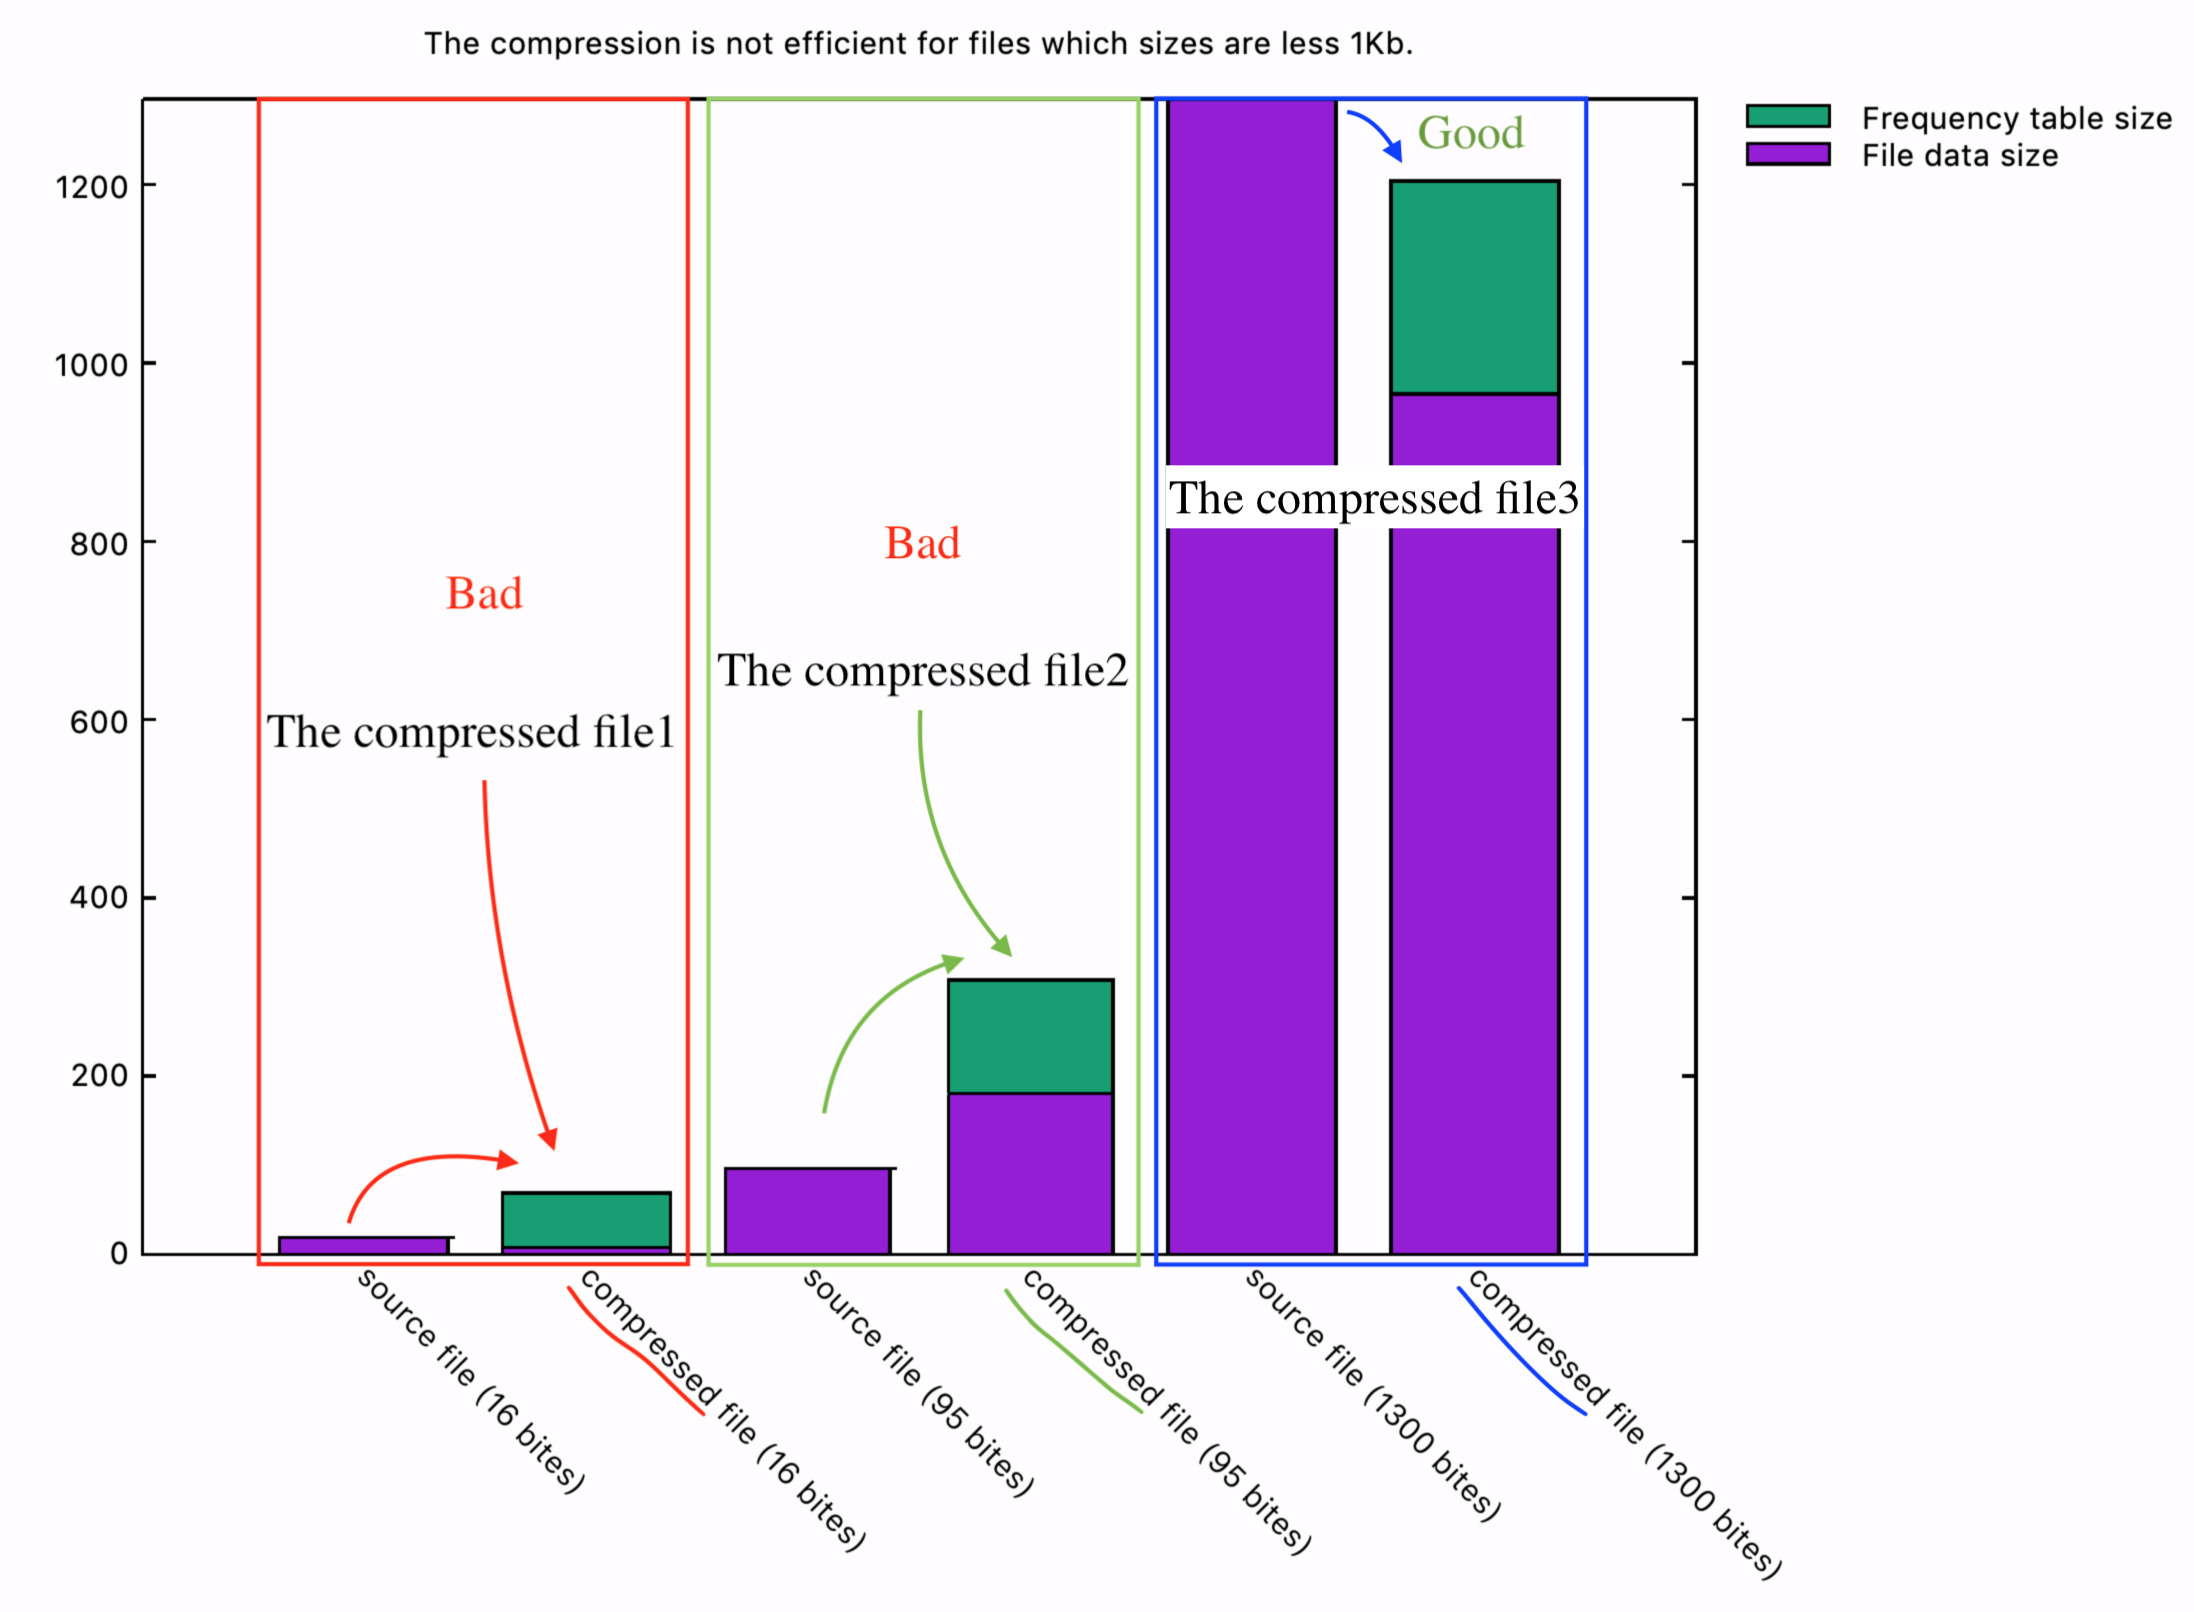
\includegraphics[width=0.85\linewidth]{\commonSecPathPrefix/sec_2/content/small_compress.png}
    \caption{Эффективность сжатия небольших файлов}
    \label{fig:compress}
\end{figure}



Опытным путем для нашей программы было установлено, что коэффициент сжатия становится меньше единицы (отношение занимаемой памяти архивированного и исходного файлов) при размере исходного файла больше 1 Кб.
Если размер файла меньше 1 Кб, то с почти стопроцентной вероятностью размер архива будет больше, чем первоначальный размер файла.
Эффективность архивации маленьких файлов наиболее наглядно представлена на рисунке \ref{fig:compress}.



Стоит понимать, что длина таблицы частот также зависит от количества символов в алфавите данных.
Например, если вся последовательность будет состоять только из букв «а» и «b», то соответственно и сама таблица будет иметь только две записи, а это значит, что и эффективность сжатия такой последовательности будет при небольшом размере исходных данных более высокой.



Рассмотрим пример: представим, что у нас есть некоторый текст, который состоит только из символов «а», «b», «c», «d» и «e», а частоты их появления равны 15, 7, 6, 6 и 5 соответственно. 
Ипользуя описанный выше алгоритм построения дерева\cite{wiki_huf}, создадим сам граф и рассмотрим формирование кодировок символов.

\begin{figure}[h]
    \centering
    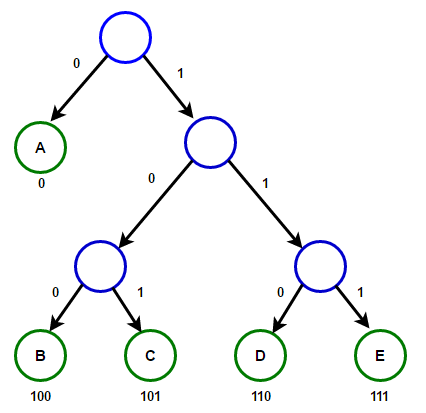
\includegraphics[height=8cm]{\commonSecPathPrefix/sec_2/content/Htree.png}
    \caption{Дерево Хаффмана для выбранного алфавита}
    \label{fig:htree}
\end{figure}



На изображении \ref{fig:htree} показаны веса соответствующих узлов и указаны соответствующие этим узлам листья со значениями символов.
Таким образом символ «а» кодируется значением 0, «b» -- 100, «c» -- 101 и так далее. 
По рисунку наглядно видно как образуется кодировка разных листьев. 
При обходе дерева в глубину, проходя по каждому узлу, кодировка символа, лежащего в нижнем листе увеличивается на один бит.
В итоге, при проходе по дереву, начиная с его корня, заканчивая листями, мы получаем кодировки всех символов, нужных нам для создания таблицы и последующей записи их в архивный файл.
В заключение стоит отметить, что для алфавита произвольной длины дерево должно иметь ровно столько же листьев, сколько и символов в данном алфавите.